\newpage
\section{Datová sada}
\label{sec:mnist}
Datová sada MNIST se skládá z černobílých obrázků \textbf{ručně psaných} číslic o velikosti $28~\times~28$~px.
Každá číslice je vycentrovaná a má konzistentní velikost\footnote{Normalizace za účelem lepší rozpoznatelnosti.}.
Vzorky MNIST číslic představuje \autoref{fig:mnist_example}.
MNIST obsahuje 60 000 obrázku pro trénování a 10 000 obrázků pro testování.

\begin{figure}[H]
    \centering
    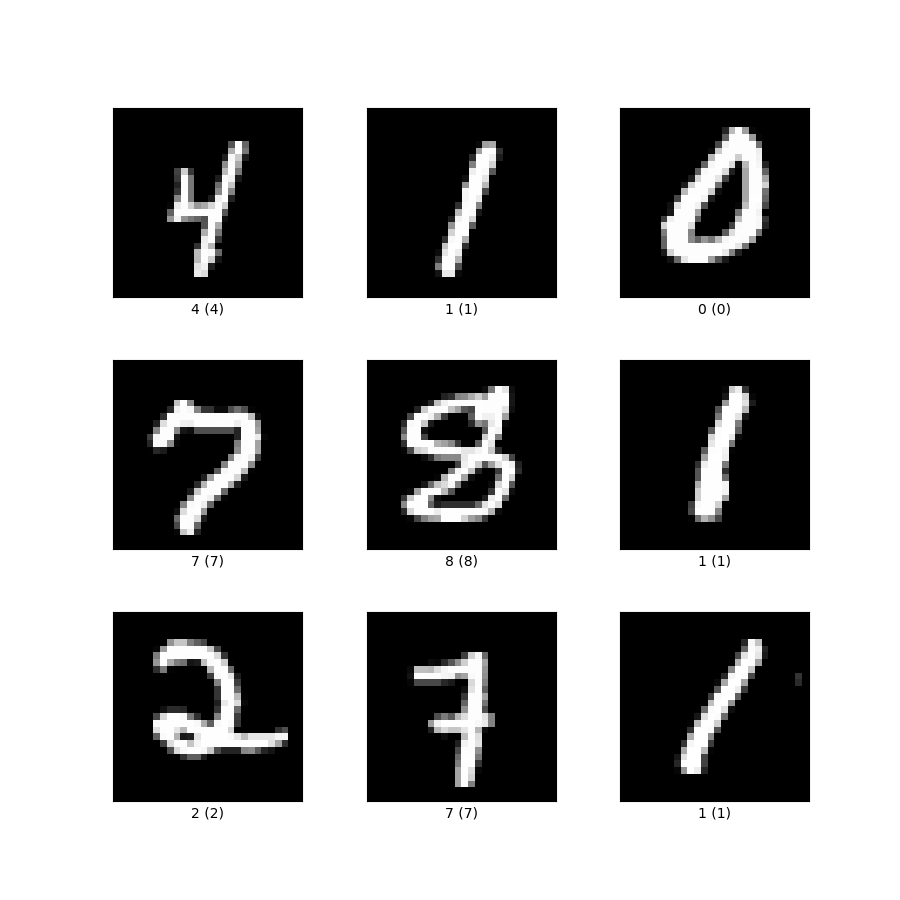
\includegraphics[width=0.45\textwidth]{figures/mnist_example.png}
    \caption{Ukázka vzorků z MNIST.}
    \label{fig:mnist_example}
\end{figure}

Datová sada je dostupná z \textcite{LeCun2010}. Datová sada MNIST se díky své jednoduchosti často využívá pro ilustrační implementace modelů strojového učení, a i z tohoto důvodu byl pro tuto kapitolu zvolen.
